\documentclass{article}
\usepackage[margin=1in]{geometry}
\usepackage{amsmath}
\usepackage{booktabs}
\usepackage{float}
\usepackage{graphicx}
\usepackage{tikz}
\usetikzlibrary{arrows.meta}
\usepackage[hidelinks]{hyperref}

\title{Superscalar Pipeline and Branch Prediction}
\author{}
\date{}

\begin{document}
\maketitle


\section{Pipeline Design}
We implemented a five-stage timing simulator with fetch, decode, execute, memory access, and writeback. The pipeline width is configurable. Instructions come from a committed-path trace, so the simulator tracks when instructions can advance without computing their register values.

Decode checks source registers and condition codes against older instructions. For a multi-lane pipeline, this includes older instructions in the same group. If an instruction stalls, younger instructions wait behind it. Processing writeback before decode makes a register written in the current cycle available to decode.

Execute and memory forwarding can be enabled separately. An ALU result can be forwarded from execute, but a load result is not available until memory access. Forwarding therefore removes some dependence stalls while leaving load-use stalls when the value has not arrived.


\begin{figure}[H]\centering
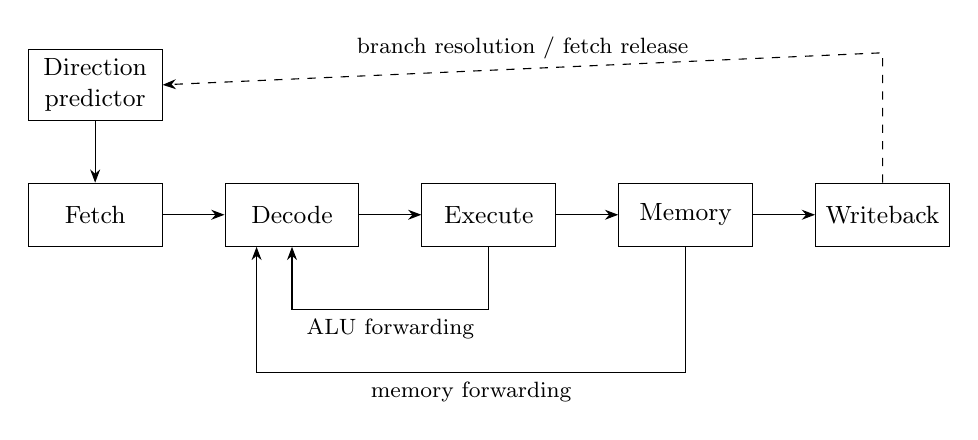
\begin{tikzpicture}[>=Stealth, font=\small, block/.style={draw, minimum width=1.7cm, minimum height=.8cm, align=center}]
\node[block] (if) at (0,0) {Fetch};
\node[block] (id) at (2.5,0) {Decode};
\node[block] (ex) at (5,0) {Execute};
\node[block] (mem) at (7.5,0) {Memory};
\node[block] (wb) at (10,0) {Writeback};
\draw[->] (if) -- (id); \draw[->] (id) -- (ex);
\draw[->] (ex) -- (mem); \draw[->] (mem) -- (wb);
\draw[->] (ex.south) -- ++(0,-.8) -| node[pos=.25,below,font=\footnotesize]{ALU forwarding} (id.south);
\draw[->] (mem.south) -- ++(0,-1.6) -| node[pos=.25,below,font=\footnotesize]{memory forwarding} ([xshift=-.45cm]id.south);
\node[draw,align=center,minimum width=1.7cm] (bp) at (0,1.65) {Direction\\predictor};
\draw[->] (bp.south) -- (if.north);
\draw[->,dashed] (wb.north) -- ++(0,1.65) -- node[above,font=\footnotesize]{branch resolution / fetch release} (bp.east);
\end{tikzpicture}

\caption{Five-stage pipeline. Solid return paths show selectable forwarding; the dashed path shows branch resolution.}\label{fig:architecture}
\end{figure}

\section{Branch Prediction}
We compared perfect prediction, always taken, and gshare. Gshare uses a 12-bit global history register and 4,096 two-bit counters, initially weakly taken. The table index is
\[
I=(PC\mathbin{\&}\texttt{0xFFF})\oplus GHR.
\]
After a branch resolves, its counter is updated toward the actual outcome and the history register is shifted. A misprediction stops fetch until the branch reaches writeback. No wrong-path instructions are inserted into the trace.

\section{Results}
Table~\ref{tab:pipeline} gives CPI for each pipeline configuration. Scalar and Dual use widths one and two without forwarding. Forwarding uses width two with both forwarding paths. These three runs use perfect prediction. Taken and Gshare use the same forwarded two-wide pipeline.

\begin{table}[H]\centering\small
\begin{tabular}{lrrrrr}
\toprule
Workload & Scalar & Dual & Forwarding & Taken & Gshare \\
\midrule
bzip2 & 1.062 & 0.578 & 0.508 & 0.662 & 0.515 \\
gcc & 1.141 & 0.672 & 0.521 & 0.612 & 0.525 \\
libq & 1.182 & 0.727 & 0.545 & 0.545 & 0.545 \\
mcf & 1.363 & 1.018 & 0.658 & 0.796 & 0.661 \\
sml & 1.220 & 0.770 & 0.570 & 0.800 & 0.800 \\
\bottomrule\end{tabular}\caption{CPI for the pipeline configurations.}\label{tab:pipeline}\end{table}

\begin{figure}[H]\centering
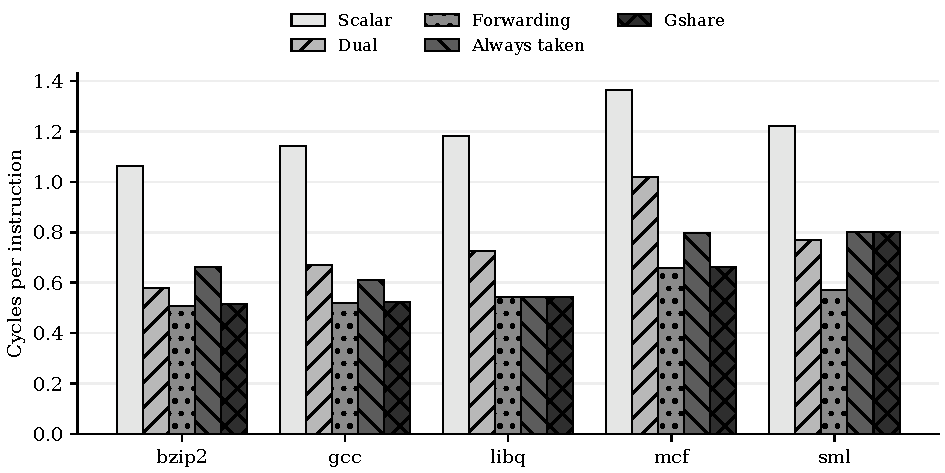
\includegraphics[width=\linewidth]{figures/cpi.pdf}
\caption{CPI by pipeline configuration. Forwarding, always taken, and gshare use a two-wide pipeline with both forwarding paths.}\label{fig:results}
\end{figure}

For gcc, increasing width reduces CPI from 1.141 to 0.672. Forwarding lowers it to 0.521, giving a $1.141/0.521=2.19$ speedup over the scalar configuration. On mcf, forwarding reduces CPI from 1.018 to 0.658. It still stays above the ideal two-wide CPI of 0.5 because dependent instructions cannot always advance together.

Gshare reduces branch mispredictions from 43.160\% to 2.033\% on bzip2, from 27.503\% to 1.330\% on gcc, and from 24.900\% to 0.568\% on mcf. Their CPI values are then close to the perfect-prediction results.

The sml trace has only 100 instructions and 15 conditional branches. Both predictors miss seven branches and produce 0.800 CPI.

The simulator measures pipeline timing with fixed stage behavior. Cache misses and branch-target prediction are not modeled. The pipeline sweep script reruns these configurations.


\end{document}
